%%%%%%%%%%%%%%%%%%%%%%%%%%%%%%%%%%%%%%%%%%%%%%%%%%%%%%%%%%%%%%%%%%%%%%%%%%%%%%%%
% \documentclass[12pt,papel,twoside]{ibtesis}
%\documentclass[12pt,screen,twoside,pagebackref]{ibtesis}
 \documentclass[12pt,papel,singlespace,oneside]{ibtesis}
% \documentclass[12pt,papel,preprint,singlespace,oneside]{ibtesis}
%%%%%%%%%%%%%%%%%%%%% Paquetes extra %%%%%%%%%%%%%%%%%%%%%%%%%%%%%%%%%%%%%%%%%%%
% Por conveniencia: aqu\'{\i} puede cargar todos los paquetes y definir los comandos 
% que necesite
\usepackage{ibextra}
\usepackage{subfig} %para poner varias imagenes en una sola figura
\usepackage{url} %para citar páginas web
\usepackage{notoccite}
\usepackage{verbatim} 
%\nofiles
%%%%%%%%%%%%%%%%%%%%%%%%%%%%%%%%%%%%%%%%%%%%%%%%%%%%%%%%%%%%%%%%%%%%%%%%%%%%%%%%
%%%%%%%%%%%%%%%%%%%%% Informacion sobre la tesis %%%%%%%%%%%%%%%%%%%%%%%%%%%%%%%
\title{Desarrollo de Texturas: Integraci\'on de la Microestructura mediante Experimentos y Simulaciones}
\author{Mgtr. Emanuel Alejandro Benatti}
\director{Dr. Raúl Eduardo Bolmaro}
\carrera{Tesis Doctorado en F\'{\i}sica}
\grado{Doctorando}
\laboratorio{Física y Micromecánica de materiales heterogéneos \\ Instituto de Física Rosario}
%\palabrasclave{DETECTOR, SUPERCONDUCTOR, MgB$_{2}$, NEUTRÓN}
%\keywords{detector, superconductor, MgB$_{2}$, neutron}
% Si queremos poner la fecha manualmente:
% \date{Diciembre de 2099}

%%%%%%%%%%%%%%%%%%%%%%%%%%%%%%%%%%%%%%%%%%%%%%%%%%%%%%%%%%%%%%%%%%%%%%%%%%%%%%%%
%\titlepagefalse % Si no quiere compilar la portada descomente esta linea
%\includeonly{apendices} % Compilar s\'{o}lo estos archivos 
%\graphicspath{{figs/}} % Lugar donde encontrar las figuras generales (se puede poner uno en cada cap{\'{\i}}tulo)
%%%%%%%%%%%%%%%%%%%%%%%%%%%%%%%%%%%%%%%%%%%%%%%%%%%%%%%%%%%%%%%%%%%%%%%%%%%%%%%%


\begin{document}

% Dentro del environment 'preliminary' va:
% la dedicatoria, resumen, abstract, indices

\begin{preliminary}

% Escriba su dedicatoria
\dedicatoria{
A mi familia\\
A mis amigos\\
y a todos los que se lo merecen \\
por merecerlo. \\
}

%%% \'{I}ndices %%%%
%\begin{abreviaturas}
%    \printnomenclature
%\end{abreviaturas}

\tableofcontents                %\'{I}ndice

\listoffigures                  %Figuras

%\listoftables                   %Tablas

\listofabbr						%Símbolos y abreviaturas


\begin{resumen}%
  En este trabajo se estudia la viabilidad de utilizar films del supuerconductor MgB$_2$, que tiene una temperatura crítica alrededor de 39\,K, para construir un detector de neutrones térmicos y fríos. El objetivo es aprovechar el calor generado por la reacción $^{10}$B$(n,\alpha)^6$Li que tiene una sección eficaz de 3800\,barns para neutrones térmicos y libera una energía de aproximadamente 2.3\,MeV. El calor producido por la reacción produce una supresión momentánea de la superconductividad, lo que produce una señal que permite registrar la captura de un neutrón. Se realizaron simulaciones de las trayectorias de los productos de la reacción en el MgB$_2$ para estimar las dimensiones del detector que permitan maximizar su señal, sensibilidad y eficiencia, y que minimicen el tiempo de respuesta, al tiempo que se estimó que la energía de la reacción se deposita en un volumen de unos pocos micrómetros cúbicos. Cálculos y simulaciones hechas con el software comercial de elementos finitos COMSOL MULTIPHYSICS llevaron a la conclusión de que para poder detectar eficientemente neutrones con el MgB$_2$, resulta necesario construir un cable que tenga un ancho no mayor a un micrón y un espesor no mucho mayor a los 200\,nm. Dimensiones mayores incrementan la probabilidad de captura de un neutrón pero reducen drásticamente la señal y la sensibilidad del detector, además de que dificultan el control de la temperatura del mismo.

Fueron realizadas simulaciones en las que se acopló la física del comportamiento térmico y eléctrico del detector, y se observó que si el mismo es operado con corrientes lo suficientemente bajas, la señal y el tiempo de respuesta del detector no se modifican, y que tiene un tiempo de respuesta de algunos nanosegundos cuando el espesor del cable es de 200\,nm. También se llevaron a cabo simulaciones intentando regular la temperatura del detector simplemente variando la tensión aplicada al mismo, pero el resultado fue que eso no es posible desde el punto de vista práctico, ya que para regular la temperatura del detector en el rango de interés, es preciso aplicar tensiones que llevan a que circulen corrientes enormes por el cable de MgB$_2$. La conclusión extraída de este cálculo fue que el detector va a requerir un mecanismo adicional para controlar su temperatura. También se concluyó que por razones de estabilidad en el control de la misma, es conveniente operar al detector a tensión constante, en vez de hacerlo a corriente constante.

En conjunto con el trabajo de las simulaciones se intentó crecer films de MgB$_2$ por medio de dos técnicas diferentes, una utilizando un método ex-situ que requrió temperaturas del orden de los 700\,$^{\circ}$C, y otra consistente en un método in-situ que requería temperaturas iban de los de 500\,$^{\circ}$C hasta temperatura ambiente.

La primera técnica de crecimiento consistió en depositar films de B por evaporación para luego recocer los mismos junto con pastillas de MgB$_2$ bulk en ampollas de cuarzo. Se lograron fabricar films de un espesor de algunos cientos de nanómetros, cuyas curvas de magnetización, medidas en un magnetómetro SQUID, presentaron irreversibilidades en un ciclo \textit{Zero Field Cooling - Field Cooling} compatibles con la formación de una fase superconductora. Sin embargo, siguiendo este método no se pudo conseguir fabricar films con una transición superconductora lo suficientemente estrecha como para poder fabricar el detector, lo que probablemente se debió a que el sustrato reaccionaba con el film debido a las elevadas temperaturas del recocido.

La segunda técnica de crecimiento de films de MgB$_2$ explorada en este trabajo fue la de crecimiento directo de films por sputtering, a partir de un blanco de MgB$_2$ obtenido comercialmente. Se realizaron estudios de difracción de rayos X que no mostraron la formación de la fase MgB$_2$. Un estudio de la composición de los films crecidos fue realizado utlizando espectroscopía de rayos X caracterísiticos (EDX) y retrodispersión de Rutherford (RBS). Ambos estudios mostraron que los films crecidos tienen un exceso de B, lo que probablemente sea la causa de que no sean superconductores, tal como mostraron las mediciones de magnetización realizadas sobre las muestras. Se decidió intentar recocer los films crecidos con pastillas de Mg, en busca de mejorar la proporcion B/Mg de los films utilizando una temperatura de recocido más baja que la empleada con los films crecidos por evaporación. El recocido logró una mejora en las propiedades de transporte de las muestras, ya que pasaron de ser aislantes a ser semiconductoras, pero no se pudo observar la formación de fases superconductoras, ni en mediciones de magnetización, ni en mediciones de transporte, lo que consituye un indicio de que los films no lograron incorporar la cantidad suficiente de Mg como para volverse superconductores. Esto último se deba probablemente a que la temperatura de recocido no fue lo suficientemente alta como para permitir la difusión de la cantidad necesaria de Mg a través del film.
\end{resumen}

\begin{abstract}%
	In this paper we study the feasibility of using films of the superconductor MgB$_2$ with a critical temperature of 39\,K, to build a cold neutron and thermal neutron detector. The aim is to use the heat generated by the reaction $^{10}$B$(n,\alpha)^6$Li which has a cross section of 3800\,barns for thermal neutrons and releases an energy of approximately 2.3\,MeV. The heat produced by the reaction causes a partial destruction of superconductivity. One then notices the appearance of a single neutron by the electric resistance variation of the MgB2 thin film. Simulations of the trajectories of the reaction products in the MgB$_2$ were performed for estimating the optimal detector dimensions. Calculations and simulations with the commercial software COMSOL Multiphysics led to the conclusion that in order to efficiently detect neutrons with MgB$_2$, is necessary to build a cable that has a width no greater than one micron and a thickness not much greater than 200\,nm. Larger dimensions increase the probability of neutron capture but drastically reduces the produced signal and the detector sensitivity, plus it difficult the temperature control of the device.

	Simulations were also conducted coupling the physics of the thermal and electrical behavior of the detector, and it was found that if it is operated with a small bias-current, the detector's signal and response time are not changed. Calculations showed that the detector has a response time of few nanoseconds for a wire 200\,nm thick. Simulations were carried out trying to regulate the temperature of the detector by varying the bias tension, but it was found that this is not a viable option from a practical standpoint, as to regulate the temperature of the detector in the range of interest, it is necesary to apply voltages that lead to large currents circulating through the detector. This implied that the construction of the detector will require an additional mechanism to control its temperature. It was also found that for reasons of stability in temperature control, it is desirable to operate the detector voltage-biased instead of current-biased.

	In addition with the simulations, growth of MgB$_2$ films was attempted by two different means, one using an ex-situ method requiring temperatures around 700\,$^{\circ}$C, and an in-situ method requiring temperatures of 500\,$^{\circ}$C down to room temperature.

	The first technique consisted on growing of boron films by evaporation and a post-annealing process with a bulk MgB$_2$ sample in a quartz tube. We managed to make 200\,nm thick films, and perform magnetization measurements in a SQUID magnetoteter. Irreversibilities shown in a Zero Field Coolig - Field Coolig magnetization measurement were compatible with the formation of a superconducting phase. However, it wasn't possible to obtain films with a sharp superconducting transition, as it's needed to build the detector. This is probably the result of a chemical reaction between substrate and the film due to the high annealing temperatures.

  The second technique explored in this work was the direct growth of MgB$_2$ films by sputtering. To this end a commercial MgB$_2$ target was used. Studies performed by X-ray diffraction did not show the formation of the MgB$_2$ crystalline phase. We also studied the composition of the films by electron dispersive X-ray analisys (EDX) and Rutherford backscattering (RBS). Both studies showed that films are grown with an excess of B, which is probably the reason why they are not superconducting, as was observed by magnetization measurements. Films were annealed with Mg pellets, seeking to increase the amount of Mg in the films, using lower annealing temperatures than those used with the films grown by evaporation. Samples showed an improvement in their transport properties after the annealing, as they went from being insulating to semiconductonducting. However no formation of a superconducting phase was observed, neither in magnetization measurements or in electrical resistance measurements. This is probably due to the low annealing temperature, which did not allow the diffusion of the required amount of Mg through the film.
\end{abstract}

%%% Local Variables: 
%%% mode: latex
%%% TeX-master: "template"
%%% End: 

\end{preliminary}


% Podemos usar cualquiera de los dos comandos: \input o \include para incluir el texto
\chapter{Introducci\'on}
\graphicspath{{./figs/01_intro/}}
\chapterquote{La destrucción es obra de una tarde. La creación es obra de una vida.}{Kamahl, acólito druida}
\section{Motivación}\label{S:motivacion}
\cite{Mainprice2011}
\section{Difracción de Rayos X}\label{S:DRX}
Los rayos X son una herramienta de vital importancia para el estudio de los materiales cristalinos. 
En la difracción de Rayos X (DRX), un haz monocromático de de rayos X de longitud de onda $\lambda$ incide sobre una dada muestra (Fig. \ref{fig:Bragg}). 
Si el cristal es infinito y está libre de cualquier tipo de distorsiones, para una dada familia de planos ${hkl}$, habrá interferencia constructiva para los haces salientes que cumplan con la condición de Bragg[ref]:

Esto esta medio medio, hay que hablar de que los cristales estan en arreglos periodicos de atomos

\begin{equation}
  2 \ d_{hkl} \ \sin(\theta_{B}) \ = \ n \ \lambda
  \label{eq:Bragg}
\end{equation}
\noindent
siendo $d_{hkl}$ la distancia interplanar de la familia de planos $\{hkl\}$, 2$\theta_{B}$ el ángulo formado entre el haz incidente y el haz reflejado y $n$ el número de orden de difracción. 

Hay que pensar en el planteo mas riguroso, usando los vectores K, porque lo voy a necesitar para explicar williamson hall

\nomenclature{$\lambda$}{Longitud de onda}
\nomenclature{$d_{hkl}$}{Distacia interplanar para la familia de planos $hkl$}
\nomenclature{$\theta_B$}{Ángulo de Bragg}
\nomenclature{XRD}{Difracción de Rayos X}
\begin{figure}[htb!]
  \centering
  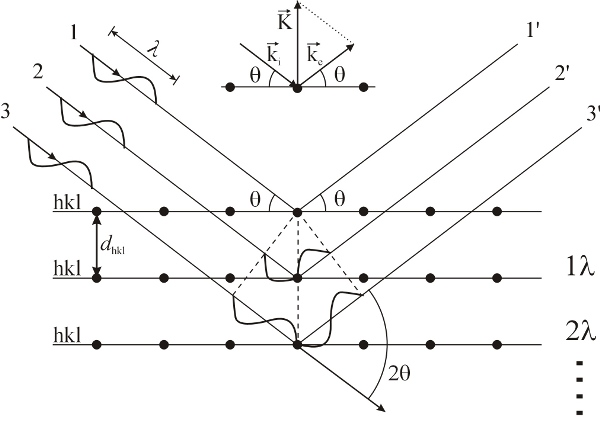
\includegraphics[width=\imsize]{BraggLaw}
  \caption{Ley de Bragg}
  \label{fig:Bragg}
\end{figure}

Una consecuencia de la ley expresada en la Ec. \ref{eq:Bragg} es que para un cierto haz incidente habrá reflexiones cuyas distribución de intensidades serán funciones deltas de Dirac[ref], con intensidad infinita para el ángulo $\theta_{B}$ e intensidad nula para los ángulos $\theta$ que no cumplan con la condición de Bragg. Como resultado, los "picos" de difracción tendrán además un ancho nulo. 
Si, como ocurre en la práctica, el número de planos que contribuyen a la reflexión es finito, la distribución angular de intensidades tendrán un ancho y altura finitos, y lo mismo ocurrirá si la red de átomos tiene distorsiones, es decir, si los átomos no se encuentran en un arreglo perfectamente periódico. 
En un experimento de DRX real aparecerán además otras contribuciones que ensancharán los picos de difracción. 
Por un lado el haz incidente no será puntual ni estará constituido por haces completamente paralelos, sino que tendrá de un tamaño finito y estará comprendido entre haces que tendrán cierta divergencia angular. 
Además, el haz no será completamente monocromático, sino que estará inegrado por rayos X con longitudes de onda en un intervalo $(\lambda \ \pm \ \Delta \lambda)$. 
Todos estos factores cotribuirán a que haya haces difractados en las vecindades de $\theta_{B}$, aumentando el ancho de los picos de difracción, y serán parte crucial de la discusión en los capítulos siguientes, ya que el ensanchamiento de los picos provee información sobre la microestructura de los materiales.

\subsection{Estudios de ancho de pico}\label{SS:DRX-LPA}
Si no se tienen en cuenta los diferentes efectos instrumentales se puede afirmar que, a partir del estudio del ensanchamiento y la forma de los perfiles de intensidad de los picos de medidos en un experimento de DRX, es posible obtener información acerca de la cantidad y tipo de defectos presentes en un material, así como información microestructural como el tamaño promedio de los dominios coherentes de difracción. 
Al conjunto de t\'ecnicas y m\'etodos del campo de la cristalografía que utilizados para obtener este tipo de información se los conoce como Estudio de Ancho de Pico, o LPA, por sus siglas en inglés (Line Profile Analysis).
Aunque el término LPA fue acuñado muchos años después, la técnica, aunque rudimentaria, es tan antigua como los primeros experimentos de DRX, y fue implementada independientemente por Hull en Estados Unidos y Debye y Scherrer en Alemania. Mientras investigaba el tamaño de partículas de oro y plata en sistemas coloidales, Scherrer incluyó la ecuación que luego llevaría su nombre[ref]:

\begin{equation}
  H \ = \ 2 \sqrt{\frac{\ln(2)}{\pi}} \ \frac{\lambda}{L \ \cos(\theta_B)}
  \label{eq:Scherrer}
\end{equation}
\noindent
Donde $H$ denota el ancho del pico a la mitad de su intensidad máxima, $L$ es la longitud característica de la cristalita y el factor numérico se usa para convertir $H$ al ancho integral del pico, suponiendo que el mismo tiene forma de gaussiana. 
Los trabajos que siguieron se dedicaron a mejorar las estimaciones de tamaño y forma de las cristalitas. 
En el año 1938 [ref] Jones señaló que el perfil de intensidades medido en un experimento de DRX, $I_{exp}$ es la convolución del perfil $I_{muestra}$ que se obtendría de la muestra y el debido a todos los efectos instrumentales, $I_{inst}$, es decir:
\begin{equation}
  I_{exp} \ = \ I_{muestra} \ \otimes \ I_{inst}
  \label{eq:conv}
\end{equation}
\noindent
De esta manera, Jones logró remover las contribuciones de las líneas $K\alpha_2$ de la radiación del cobre en las mediciones de tamaño de cristalita.


\nomenclature{$H$ o $FWHM$}{Ancho de pico a media altura. También abreviado como FWHM por sus siglas en inglés (Full Witdth at Half Maximum).}
\nomenclature{$L$}{Longitud característica de la cristalita.}

Frase de Warren?
Definicion de macro, micro, meso, nano estructura?
Diferencia entre cristalita y tamaño de grano
Definicion de defectos, dislocaciones, maclas, fallas de apilamiento, bordes de grano
Separacion, al menos en la nomenclatura de familia de planos, planos, direcciones familia de direcciones

Hay que hablar de los principios de medicion, rayos X de laboratorio y de sincrotron
Estudio de ancho de pico, Langford, Williamson Hall, Warren Averbach y CMWP

\section{Difracción de electrones retro difundidos}\label{S:EBSD}
Cómo se mide y cómo se pueden relacionar las magnitudes de EBSD con las de RX
Que permite y que no permite ver en comparacion con RX

¿Hablo de TEM?
 
\section{Textura cristalográfica}\label{S:Text}
Definicion de textura, relacion con los procesos de deformacion y la microestructura.
ODF: definicion y obtencion a partir de RX y EBSD. Diferencias de los dos métodos.

\subsection{FDO y FDO generalizada}\label{SS:ODF}
Relacion entre la ODF y la ODF generalizada. Relacion de FWHM y energía de deformacion.

\section{Revisión bibliográfica y estado del arte}\label{S:RB}

\section{Organización de la tesis}\label{S:Org}


%\appendix
%\chapter{Tablas de calor específico, conductividad térmica y eléctrica utilizadas en las simulaciones por elementos finitos}\label{C:tablas}
%\chapterquote{Negociemos Don Inodoro}{Fernando de la R\'{u}a, 2001}
%\chapterquote{Smartness runs in my family.  When I went to school I was so smart my teacher was in my class for five years}{George Burns}
\graphicspath{{figs/Apendice}}
En las secciones siguientes se muestran los datos utilizados en las simulaciones por elementos finitos que se realizaron en el capítulo \ref{C:dise}. En cada tabla se indica además la fuente de información de cada propiedad física. Los datos que aparecen en este apéndice se obtuvieron a partir de digitalizar gráficas con mediciones de calor específico, conductividad térmica o eléctrica, según correspondía, con excepción de las propiedades físicas del zafiro y el calor específico del silicio, que se obtuvieron de las bibliotecas de datos del programa comercial COMSOL MULTIPHYSICS. Estos últimos datos no se muestran en forma de tabla, sino en forma de polinomios funciones de $T$, que es como aparecían en el programa.
\newpage
\section{Propiedades físicas del MgB$_2$}
\subsection*{Calor específico}
\begin{table}[h!]
  \vspace{-0.5cm}
  \centering
  \begin{tabular}{|c|c|}\hline
  	Temperatura [K]	&	Calor específico [J/(Kg K)]	\\ \hline
  	5.693	&	0.753	\\
	8.759	&	0.780	\\
	12.409	&	0.812	\\
	16.350	&	1.549	\\
	19.562	&	1.929	\\
	21.606	&	2.650	\\
	23.796	&	3.372	\\
	26.861	&	5.507	\\
	29.927	&	6.588	\\
	32.409	&	9.772	\\
	35.037	&	12.958	\\
	36.058	&	15.075	\\
	36.496	&	16.133	\\
	36.934	&	17.191	\\
	37.518	&	18.602	\\
	38.248	&	17.554	\\
	38.978	&	16.858	\\
	40.000	&	17.570	\\
	41.022	&	20.390	\\
	42.044	&	21.804	\\
	44.526	&	25.340	\\
	45.985	&	29.921	\\
	48.175	&	34.157	\\
	49.635	&	37.332	\\
	51.533	&	40.511	\\
	52.555	&	43.683	\\
	54.015	&	48.264	\\
	55.475	&	52.493	\\
	56.496	&	56.719	\\
	57.810	&	59.893	\\
	59.124	&	64.121	\\
	60.438	&	67.998	\\
	62.628	&	73.639	\\
	64.088	&	78.572	\\
	65.110	&	84.203	\\
	66.861	&	89.138	\\
	68.613	&	97.235	\\
	71.095	&	108.501	\\
	73.431	&	118.712	\\
	74.307	&	121.180	\\
	76.204	&	129.630	\\ \hline
  \end{tabular}
  %\vspace{-1cm}
  \caption[Tabla con los valores del calor específico del MgB$_2$]{Tabla con los valores del calor específico del MgB$_2$. Datos obtenidos de \cite{Bauer2001}.}
  \label{tab:cmgb2}
\end{table}

\subsection*{Conductividad térmica}
\begin{table}[h!]
  \centering
  \begin{tabular}{|c|c|}\hline
	Temperatura [K]	&	Conductividad térmica [W/(m K)]	\\ \hline
	7,500	&	1,260	\\
	13,750	&	3,900	\\
	20,000	&	6,803	\\
	25,625	&	9,639	\\
	32,500	&	12,411	\\
	36,875	&	14,193	\\
	40,000	&	14,855	\\
	41,250	&	15,515	\\
	46,250	&	16,377	\\
	50,000	&	17,566	\\
	55,625	&	18,626	\\
	61,250	&	19,554	\\
	67,500	&	20,352	\\
	73,750	&	21,084	\\
	78,750	&	21,485	\\
	84,375	&	21,887	\\
	91,875	&	22,358	\\
	100,000	&	22,763	\\
	106,875	&	22,772	\\
	110,625	&	23,172	\\
	118,750	&	23,183	\\
	134,375	&	23,203	\\
	149,375	&	23,157	\\
	159,375	&	23,236	\\
	174,375	&	23,453	\\
	185,625	&	23,600	\\
	194,375	&	23,677	\\
	204,375	&	23,690	\\
	216,250	&	23,969	\\
	230,625	&	24,382	\\
	247,500	&	24,602	\\
	260,625	&	25,146	\\
	277,500	&	25,826	\\
	292,500	&	26,174	\\ \hline
  \end{tabular}
  \caption[Tabla con los valores de la conductividad térmica del MgB$_2$.]{Tabla con los valores de la conductividad térmica del MgB$_2$. Datos obtenidos de \cite{Putti2003}.}
  \label{tab:kmgb2}
\end{table}
\newpage
\subsection*{Conductividad eléctrica}
La conductividad eléctrica del MgB$_2$ se obtuvo a partir de mediciones de resistividad obtenidas de \cite{Nagamatsu2001}. Como la conductividad eléctrica de un superconductor diverge para temperaturas que están por debajo de $T_c$, el estado superconductor se expresa por una conductividad eléctrica varios órdenes de magnitud mayor que la que tiene el material por encima de $T_c$.
\begin{table}[h!]
  \centering
  \begin{tabular}{|c|c|}\hline
	Temperatura [K]	&	Conductividad eléctrica [S/m]	\\ \hline
	4,710	&	100000000000,000	\\
	20,000	&	100000000000,000	\\
	34,960	&	100000000000,000	\\
	36,640	&	144034522,194	\\
	36,970	&	11074675,429	\\
	37,480	&	2486133,590	\\
	37,650	&	1728814,673	\\
	37,820	&	1414401,150	\\
	38,320	&	1363822,959	\\
	41,510	&	1354673,964	\\
	45,040	&	1354288,694	\\
	47,900	&	1349626,019	\\
	51,260	&	1349261,819	\\
	60,340	&	1339676,254	\\
	68,400	&	1330333,874	\\
	74,450	&	1325500,509	\\
	78,490	&	1325078,975	\\
	83,030	&	1316302,139	\\
	87,900	&	1307606,609	\\
	92,440	&	1299058,962	\\
	96,970	&	1294600,609	\\
	99,500	&	1290372,531	\\ \hline
  \end{tabular}
  \caption[Tabla con los valores de la conductividad eléctrica del del MgB$_2$.]{Tabla con los valores de la conductividad eléctrica del del MgB$_2$. Datos obtenidos de \cite{Nagamatsu2001}.}
  \label{tab:smgb2}
\end{table}
\newpage
\section{Propiedades físicas del silicio}
\subsection*{Calor específico}
Como se explicó al principio del capítulo, los valores de calor específico del silicio no se obtuvieron de tablas, sino de las librerías de propiedades físicas del programa COMSOL MULTIPHYSICS. Este programa utiliza polinomios para aproximar los valores de calor específico. El polinomio que utiliza es de la forma $p_0(T) \,=\, A_0\,+\,A_1 \times T\,+\,A_2 \times T^2\,+\,A_3 \times T^3\,+\,A_4 \times T^4\,$, y los coeficientes del polinomio dependen del intervalo de temperatura considerado. En la tabla \ref{tab:csi} se muestran los coeficientes de dicho polinomio para cada intervalo de temperatura.
\begin{table}[h!]
  %\centering
  \hspace{-1.6cm}
  \begin{tabular}{|c|c|c|c|c|c|c|}\hline
$T_{i}\,[\rm K]$	&	$T_{f}\,[\rm K]$	&	$A_0\,[\rm J/(\rm Kg\,K)]$	&	$A_1\,[\rm J/(\rm Kg\,K^2)]$	&	$A_2\,[\rm J/(\rm Kg\,K^3)]$	&	$A_3\,[\rm J/(\rm Kg\,K^4)]$	&	$A_4\,[\rm J/(\rm Kg\,K^5)]$	\\ \hline
1.0	&	7.0	&$	-4.83\,10^{-5}	$&$	7.68\,10^{-5}	$&$	-3.42\,10^{-5}	$&$	2.81\,10^{-4}	$&$	-3.13\,10^{-7}	$\\ \hline
7.0	&	20.0	&$	0.0525	$&$	-0.0396	$&$	0.0100	$&$	-7.81\,10^{-4}	$&$	3.96\,10^{-5}	$\\ \hline
20.0	&	50.0	&$	-1.81	$&$	0.762	$&$	-0.0865	$&$	0.00374	$&$	-3.33\,10^{-5}	$\\ \hline
50.0	&	293.0	&$	-82.9	$&$	2.71	$&$	0.0140	$&$	-7.98\,10^{-5}	$&$	1.08\,10^{-7}	$\\ \hline
293.0	&	900.0	&$	63.0	$&$	3.77	$&$	-0.00695	$&$	5.95\,10^{-6}	$&$	-1.91\,10^{-9}	$\\ \hline
900.0	&	1685.0	&$	769.0	$&$	0.187	$&$	-3.18\,10^{-5}	$&$	0	$&$	0	$\\ \hline
  \end{tabular}
  \caption[Tabla con coeficientes del polinomio utilizado para calcular el calor específico del silicio.]{Tabla con coeficientes del polinomio utilizado para calcular el calor específico del silicio. El polinomio propuesto es de la forma $p_0(T) \,=\, A_0\,+\,A_1 \times T\,+\,A_2 \times T^2\,+\,A_3 \times T^3\,+\,A_4 \times T^4$. Datos obtenidos de la biblioteca de materiales del programa COMSOL MULTIPHYSICS.}
  \label{tab:csi}
\end{table}
\newpage
\subsection*{Conductividad térmica}
\begin{table}[h!]
  \centering
  \begin{tabular}{|c|c|}\hline
	Temperatura [K]	&	Conductividad térmica [$\frac{\rm W}{\rm m\ K}$]	\\ \hline
	6,897	&	0,0264	\\
	8,513	&	0,0481	\\
	10,251	&	0,0765	\\
	13,628	&	0,1292	\\
	16,821	&	0,1868	\\
	19,039	&	0,2226	\\
	21,548	&	0,2602	\\
	23,792	&	0,2926	\\
	26,928	&	0,3229	\\
	30,478	&	0,3495	\\
	35,801	&	0,3715	\\
	41,024	&	0,3655	\\
	52,553	&	0,3338	\\
	62,500	&	0,2873	\\
	75,256	&	0,2291	\\
	88,400	&	0,1724	\\
	101,299	&	0,1373	\\
	116,080	&	0,1033	\\
	158,197	&	0,0541	\\
	221,000	&	0,0289	\\
	316,476	&	0,0164	\\
	415,574	&	0,0115	\\ \hline
  \end{tabular}
  \caption[Tabla con los valores de la conductividad térmica del silicio.]{Tabla con los valores de la conductividad térmica del silicio. Datos obtenidos de \cite{Glassbrenner1964}.}
  \label{tab:ksi}
\end{table}
\newpage
\section{Propiedades físicas del zafiro}
Al igual que para el caso del calor específico del silicio, el calor específico y la  conductividad térmica del zafiro se obtuvieron a partir de polinomios en $T$, y en las tablas subsiguientes se muestran los coeficientes de dichos polinomios. El calor específico se obtuvo a partir de un polinomio del tipo $p_1(T) \,=\, A_0\,+\,A_1 \times T\,+\,A_2 \times T^2\,+\,A_3 \times T^3\,+\,A_4 \times T^4$, mientras que la conductividad térmica se calculó de un polinomio de grado 5, es decir que $\kappa_{\rm zafiro} \ \approx \ p_2(T) \,=\, A_0\,+\,A_1 \times T\,+\,A_2 \times T^2\,+\,A_3 \times T^3\,+\,A_4 \times T^4\,+\,A_5 \times T^5$.
\subsection*{Calor específico}
\begin{table}[h!]
  %\centering
  \hspace{-1.6cm}
  \begin{tabular}{|c|c|c|c|c|c|c|}\hline
$T_{i}\,[\rm K]$	&	$T_{f}\,[\rm K]$	&	$A_0\,[\rm J/(\rm Kg\,K)]$	&	$A_1\,[\rm J/(\rm Kg\,K^2)]$	&	$A_2\,[\rm J/(\rm Kg\,K^3)]$	&	$A_3\,[\rm J/(\rm Kg\,K^4)]$	&	$A_4\,[\rm J/(\rm Kg\,K^5)]$	\\ \hline
10.0	&	60.0	&$	-0.392	$&$	0.0802	$&$	-0.00507	$&$	1.91\,10^{-4}	$&$	1.78\,10^{-17}	$\\ \hline
60.0	&	130.0	&$	30.0	$&$	-1.46	$&$	0.0191	$&$	1.12\,10^{-4}	$&$	-6.09\,10^{-7}	$\\ \hline
130.0	&	300.0	&$	-42.6	$&$	-1.40	$&$	0.0434	$&$	-1.45E\,10^{-4}	$&$	1.55\,10^{-7}	$\\ \hline
300.0	&	810.0	&$	-528	$&$	7.53	$&$	-0.0139	$&$	1.243\,10^{-5}	$&$	-4.33\,10^{-9}	$\\ \hline
810.0	&	2250.0	&$	745	$&$	0.956	$&$	-7.12\,10^{-4}	$&$	2.69\,10^{-7}	$&$	-3.85\,10^{-11}	$\\ \hline
  \end{tabular}
  \caption[Tabla con coeficientes del polinomio utilizado para calcular el calor específico del zafiro.]{Tabla con coeficientes del polinomio utilizado para calcular el calor específico del zafiro. El polinomio propuesto es de la forma $p_1(T) \,=\, A_0\,+\,A_1 \times T\,+\,A_2 \times T^2\,+\,A_3 \times T^3\,+\,A_4 \times T^4$. Datos obtenidos de la biblioteca de materiales del programa COMSOL MULTIPHYSICS.}
  \label{tab:czaf}
\end{table}

\subsection*{Conductividad térmica}
\begin{table}[h!]
  \centering
  %\hspace{-1.6cm}
  \begin{tabular}{|c|c|c|c|c|}\hline
$T_{i}\,[\rm K]$	&	$T_{f}\,[\rm K]$	&	$A_0\,[\rm J/(\rm Kg\,K)]$	&	$A_1\,[\rm J/(\rm Kg\,K^2)]$	&	$A_2\,[\rm J/(\rm Kg\,K^3)]$	\\ \hline
6.0	&	47.0	&$	-5.11	$&$	1.76	$&$	-0.167	$\\ \hline
47.0	&	108.0	&$	-422	$&$	24.9	$&$	-0.385	$ \\ \hline
108.0	&	300.0	&$	316	$&$	-2.90	$&$	0.0125	$\\ \hline
300.0	&	2073.0	&$	75.8	$&$	-0.190	$&$	2.02\,10^{-4}	$\\ \hline
-&-&-&-&-\\ \hline	
$T_{i}\,[\rm K]$	&	$T_{f}\,[\rm K]$	&	$A_3\,[\rm J/(\rm Kg\,K^4)]$	&	$A_4\,[\rm J/(\rm Kg\,K^5)]$	&	$A_5\,[\rm J/(\rm Kg\,K^6)]$ \\ \hline
6.0	&	47.0	&$	0.0127	$&$	-2.59\,10^{-4}	$&$	1.64\,10^{-6} $\\ \hline
47.0	&	108.0	&$	0.00268	$&$	-8.82\,10^{-6}	$&$	1.12\,10^{-8}	$\\ \hline
108.0	&	300.0	&$	-2.77\,10^{-5}	$&$	3.10\,10^{-8}	$&$	1.37\,10^{-11}	$\\ \hline
300.0	&	2073.0	&$	-9.79\,10^{-8}	$&$	1.78\,10^{-11}	$&$	0	$\\ \hline
  \end{tabular}
  \caption[Tabla con coeficientes del polinomio utilizado para calcular la conductividad térmica del zafiro.]{Tabla con coeficientes del polinomio utilizado para calcular la conductividad térmica del zafiro. El polinomio propuesto es de la forma $p_2(T) \,=\, A_0\,+\,A_1 \times T\,+\,A_2 \times T^2\,+\,A_3 \times T^3\,+\,A_4 \times T^4\,+\,A_5 \times T^5$. Datos obtenidos de la biblioteca de materiales del programa COMSOL MULTIPHYSICS.}
  \label{tab:kzaf}
\end{table}
%%%%%%%%%%%%%%%%%%%%%%%%%%%%%%%%%%%%%%%%%%%%%%%%%%%%%%%%%%%%%%%%%%%%%%%%


\begin{biblio}
  \bibliography{./bib/biblio,./bib/otra}
\end{biblio}

\begin{postliminary}

%\begin{seccion}{Publicaciones asociadas}
%  \begin{enumerate}
%  \item Mi primer aviso en la revista \textbf{ABC}, 1996
%  \item Mi segunda publicaci\'{o}n en la revista \textbf{ABC}, 1997
%  \end{enumerate}
%\end{seccion}

\end{postliminary}

\end{document}
